\newpage
\section{Problem 5.6}
对于$q(\bm{x})=(10x_1^2-18x_1x_2+10x_2^2)/2+4x_1-15x_2+13$

\subsection{重要参数}

\[G=\begin{bmatrix}
10&-9\\
-9&10
\end{bmatrix},\qquad \lambda_1=19,\lambda_2=1,\qquad (\dfrac {\lambda_{1}-\lambda_{2}}{\lambda_{1}+x_{2}})^2 =0.81\]

\subsection{算法伪代码}
\begin{algorithm}[h]  
\caption{Steepest-denscent method for problem(5.6)}  
\begin{algorithmic}[1]  
\STATE Given $\bm{x}^{(0)}$ and $G$
\STATE Set $\bm{p}^{(0)}=-\bm{g}^{(0)},k=0$
\WHILE {$\|\bm{g}^{(k)}\|>\epsilon$}
\STATE Set $\alpha_k=-\dfrac{{{\bm{p}^{(k)}}^T}\bm{g}^{(k)}}{{\bm{p}^{(k)}}^T\bm{G}\bm{p}^{(k)}}$
\STATE Set $\bm{x}^{(k+1)}=\bm{x}^{(k)}+\alpha_k\bm{p}^{(k)}$
\STATE Set $\bm{g}^{(k+1)}=g(\bm{x}^{(k+1)})$
\STATE Set $\bm{p}^{(k)}=-\bm{g}^{(k)}$
\STATE k=k+1
\ENDWHILE
\end{algorithmic}  
\end{algorithm}  

\subsection{计算结果展示}

\begin{figure}[H]
\centering
\subfigure{
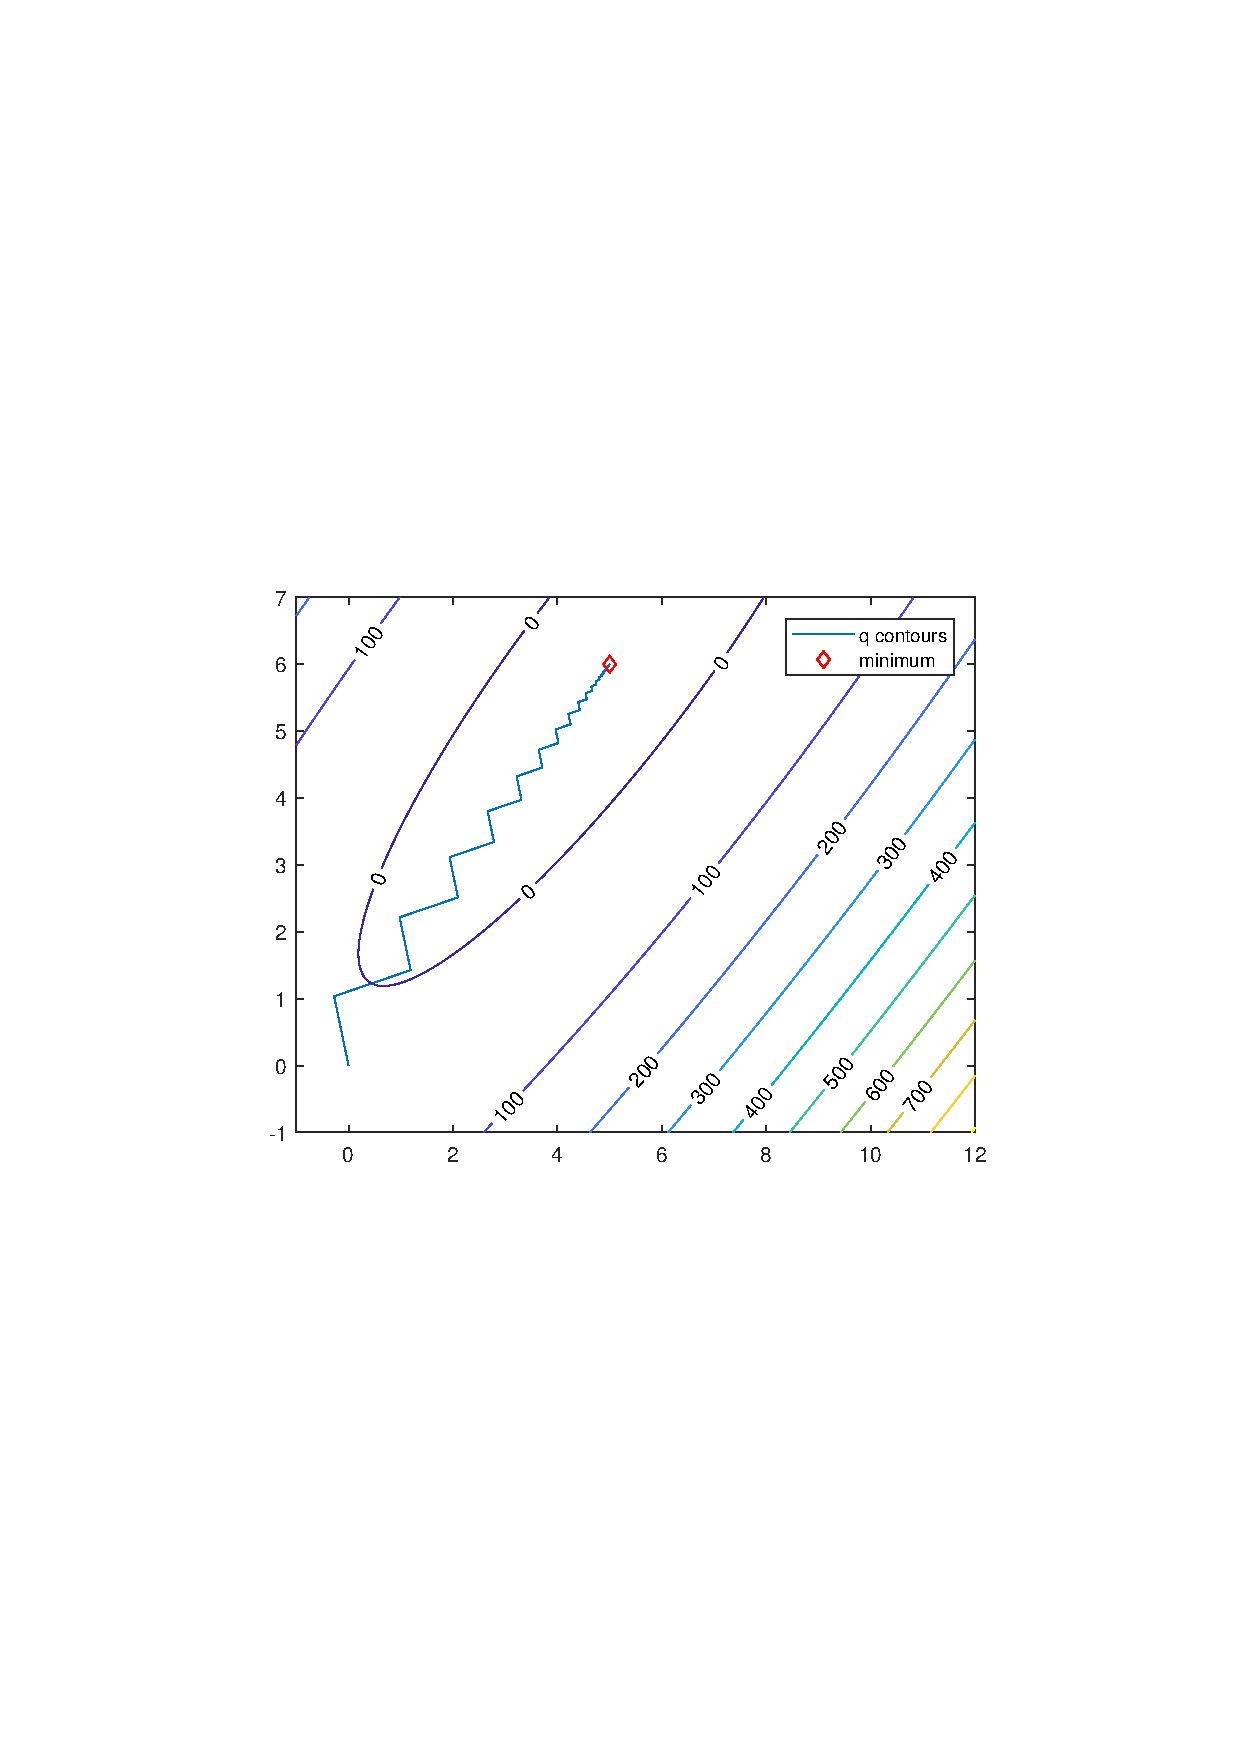
\includegraphics[width=5.7cm]{fig/1_1a.pdf}}
\subfigure{
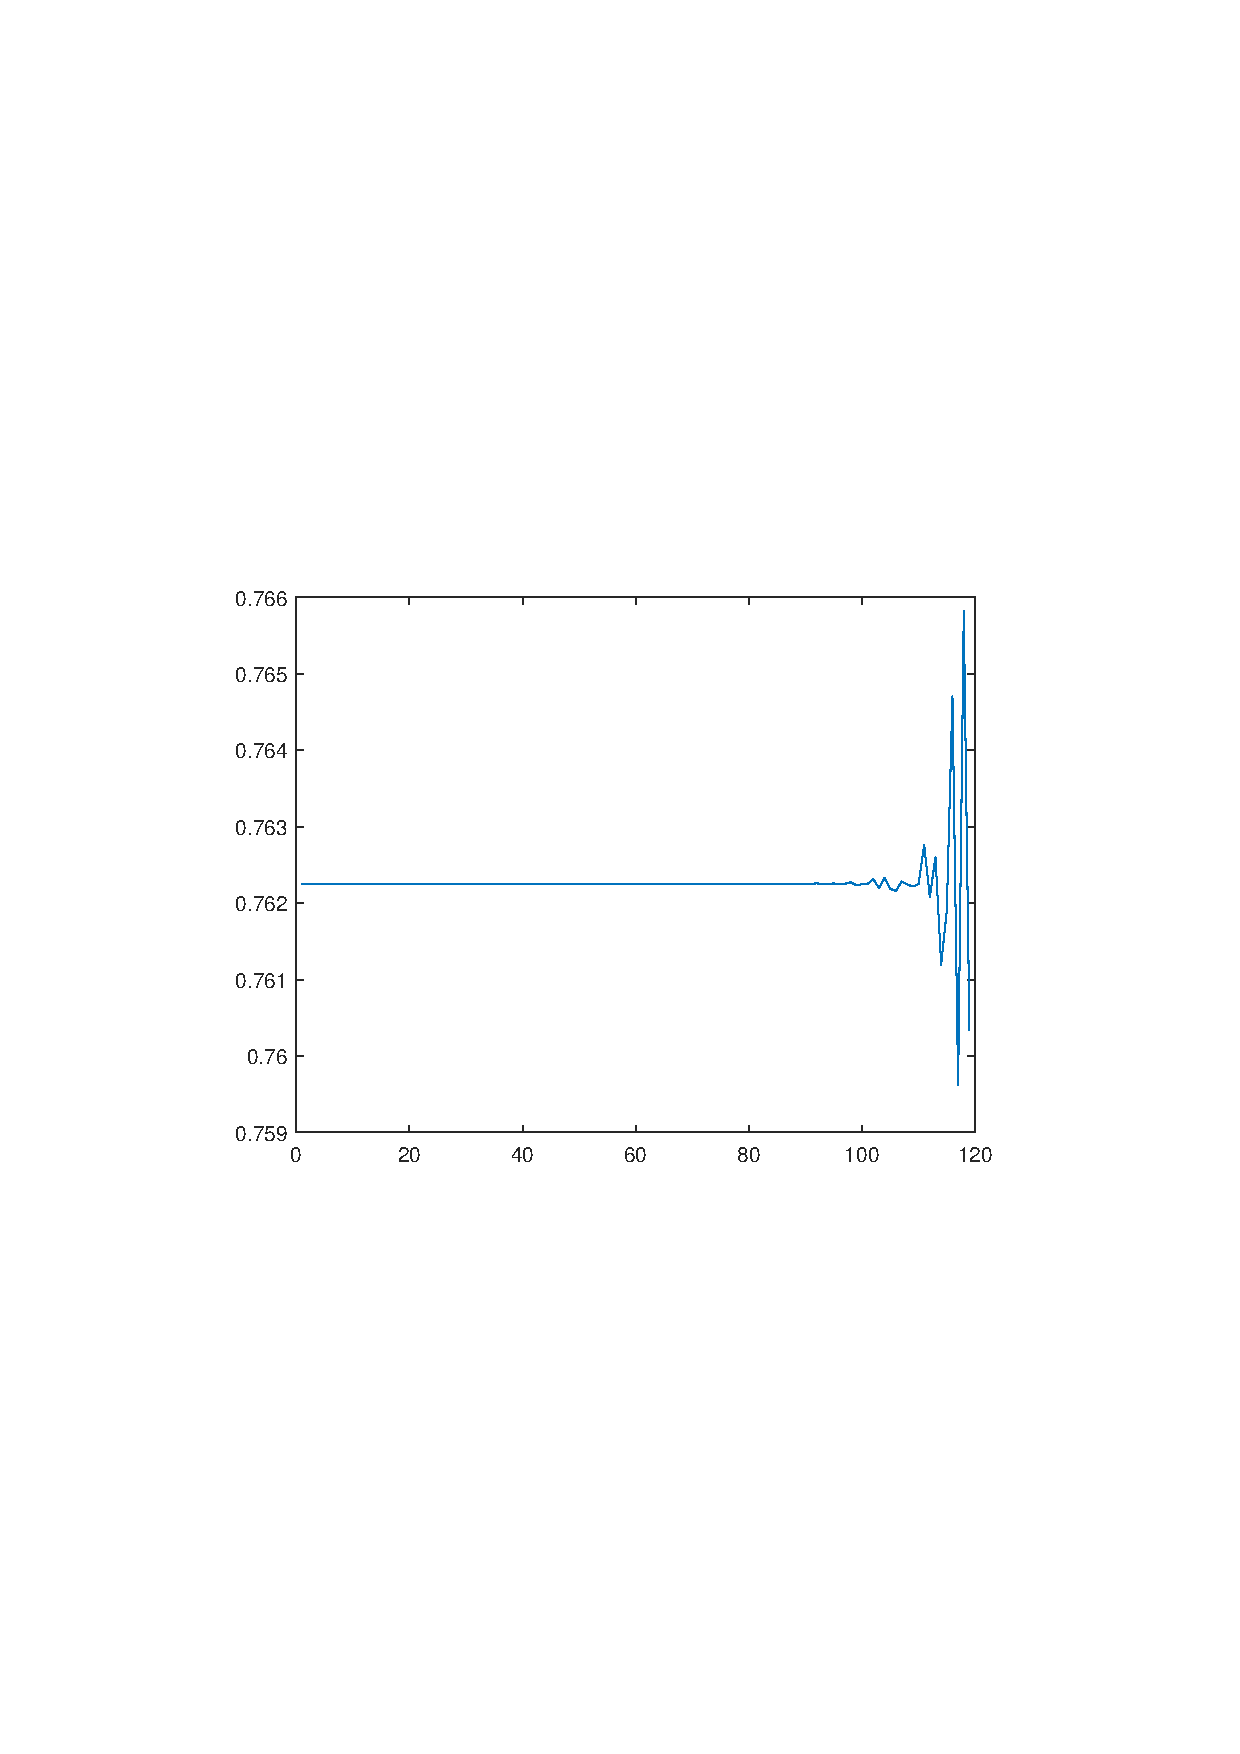
\includegraphics[width=6cm]{fig/1_1b.pdf}}
\caption{Steepest-denscent in (0,0)}
\label{Fig.lable}
\end{figure}

\begin{figure}[H]
\centering
\subfigure{
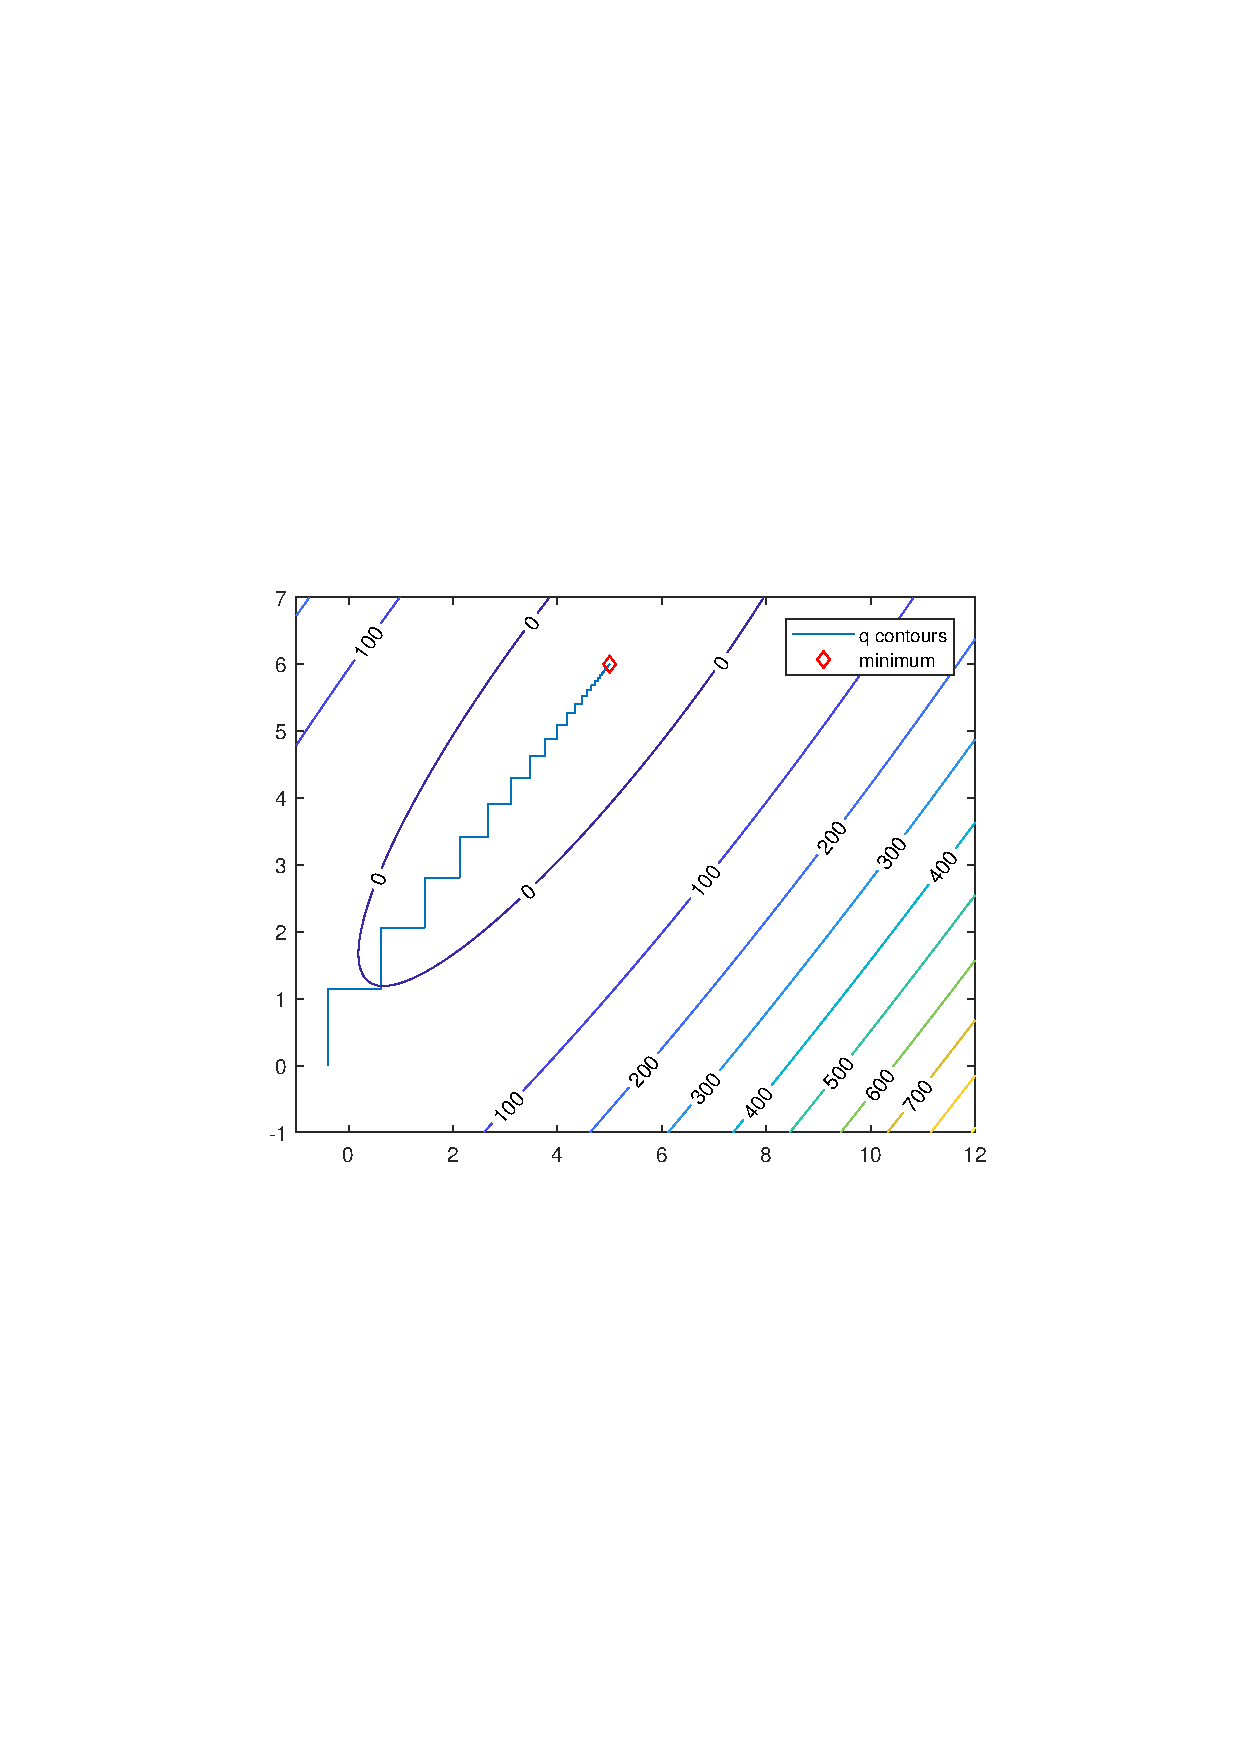
\includegraphics[width=5.7cm]{fig/1_2a.pdf}}
\subfigure{
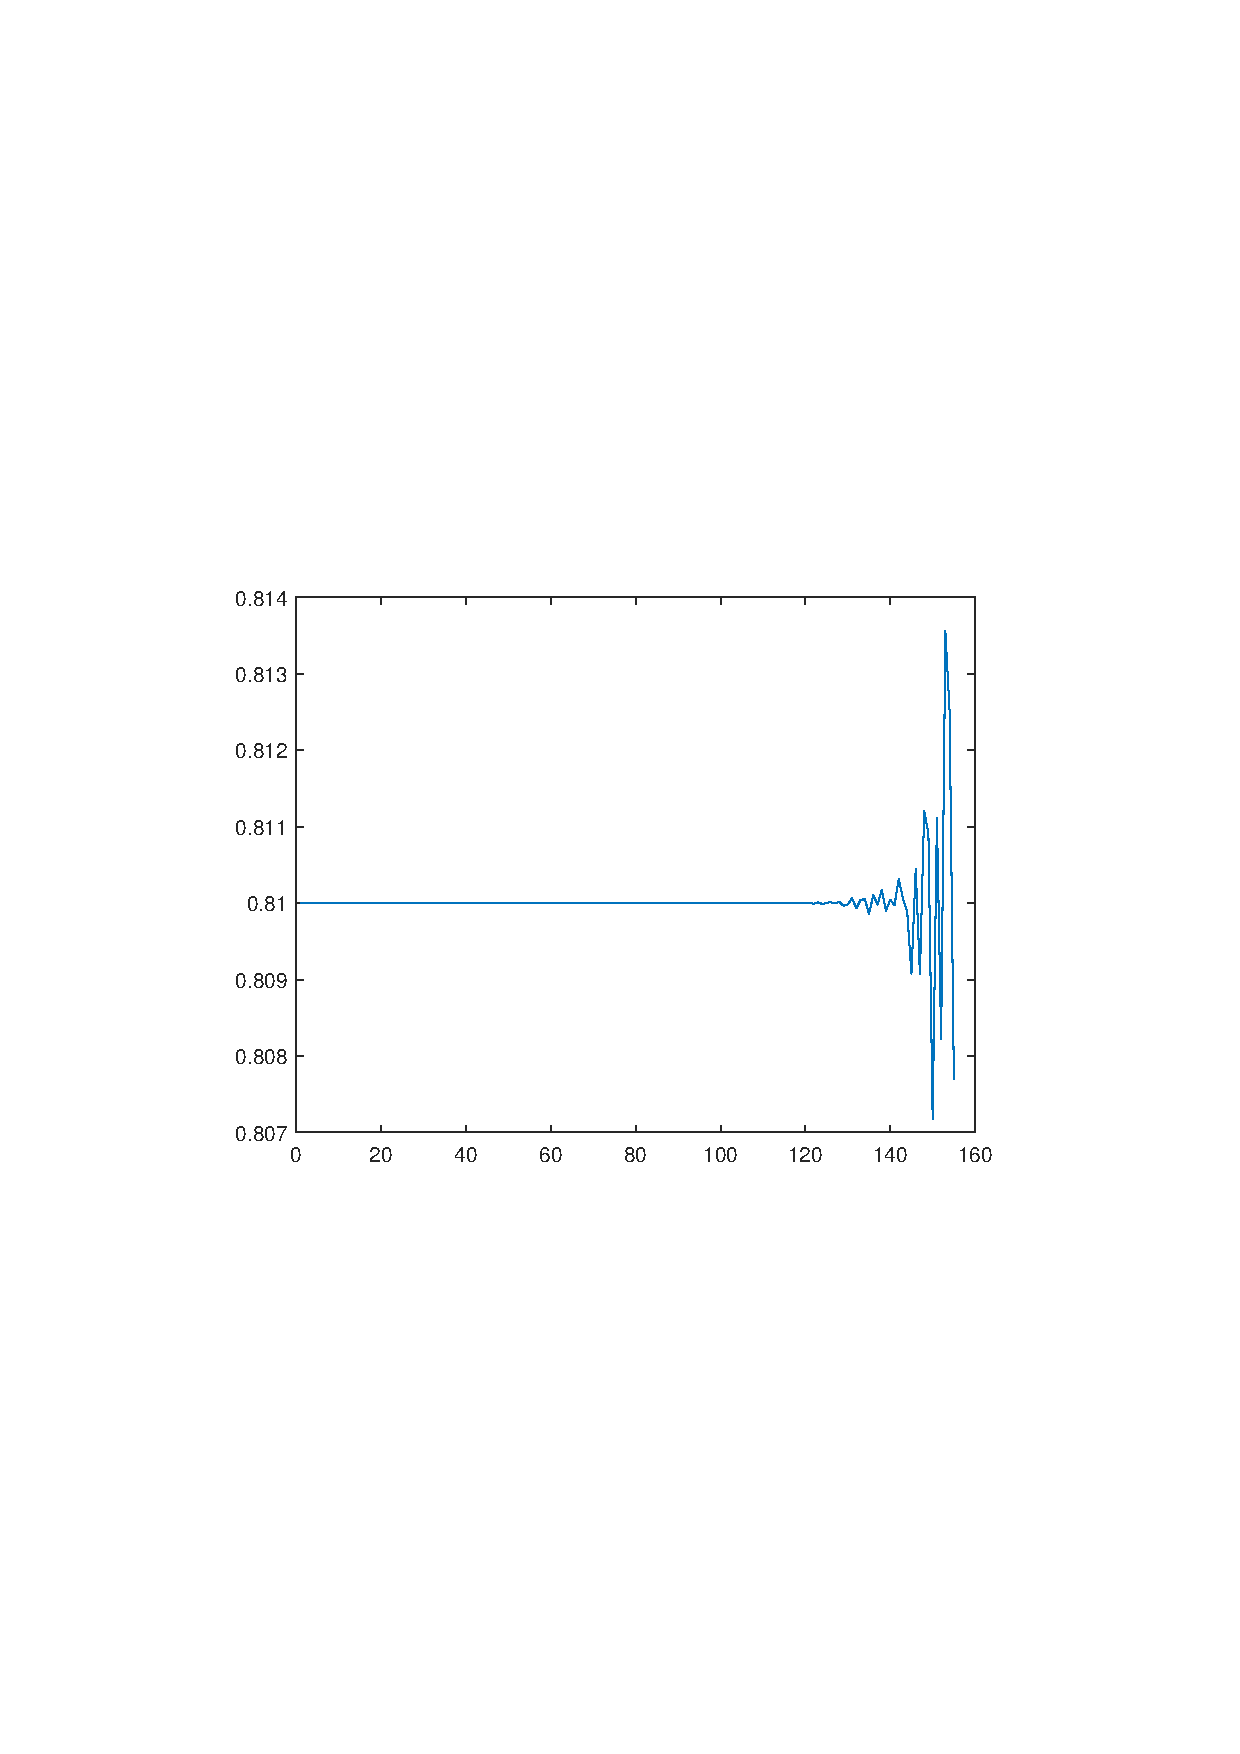
\includegraphics[width=6cm]{fig/1_2b.pdf}}
\caption{Steepest-denscent in (-0.4,0)}
\label{Fig.lable}
\end{figure}

\begin{figure}[H]
\centering
\subfigure{
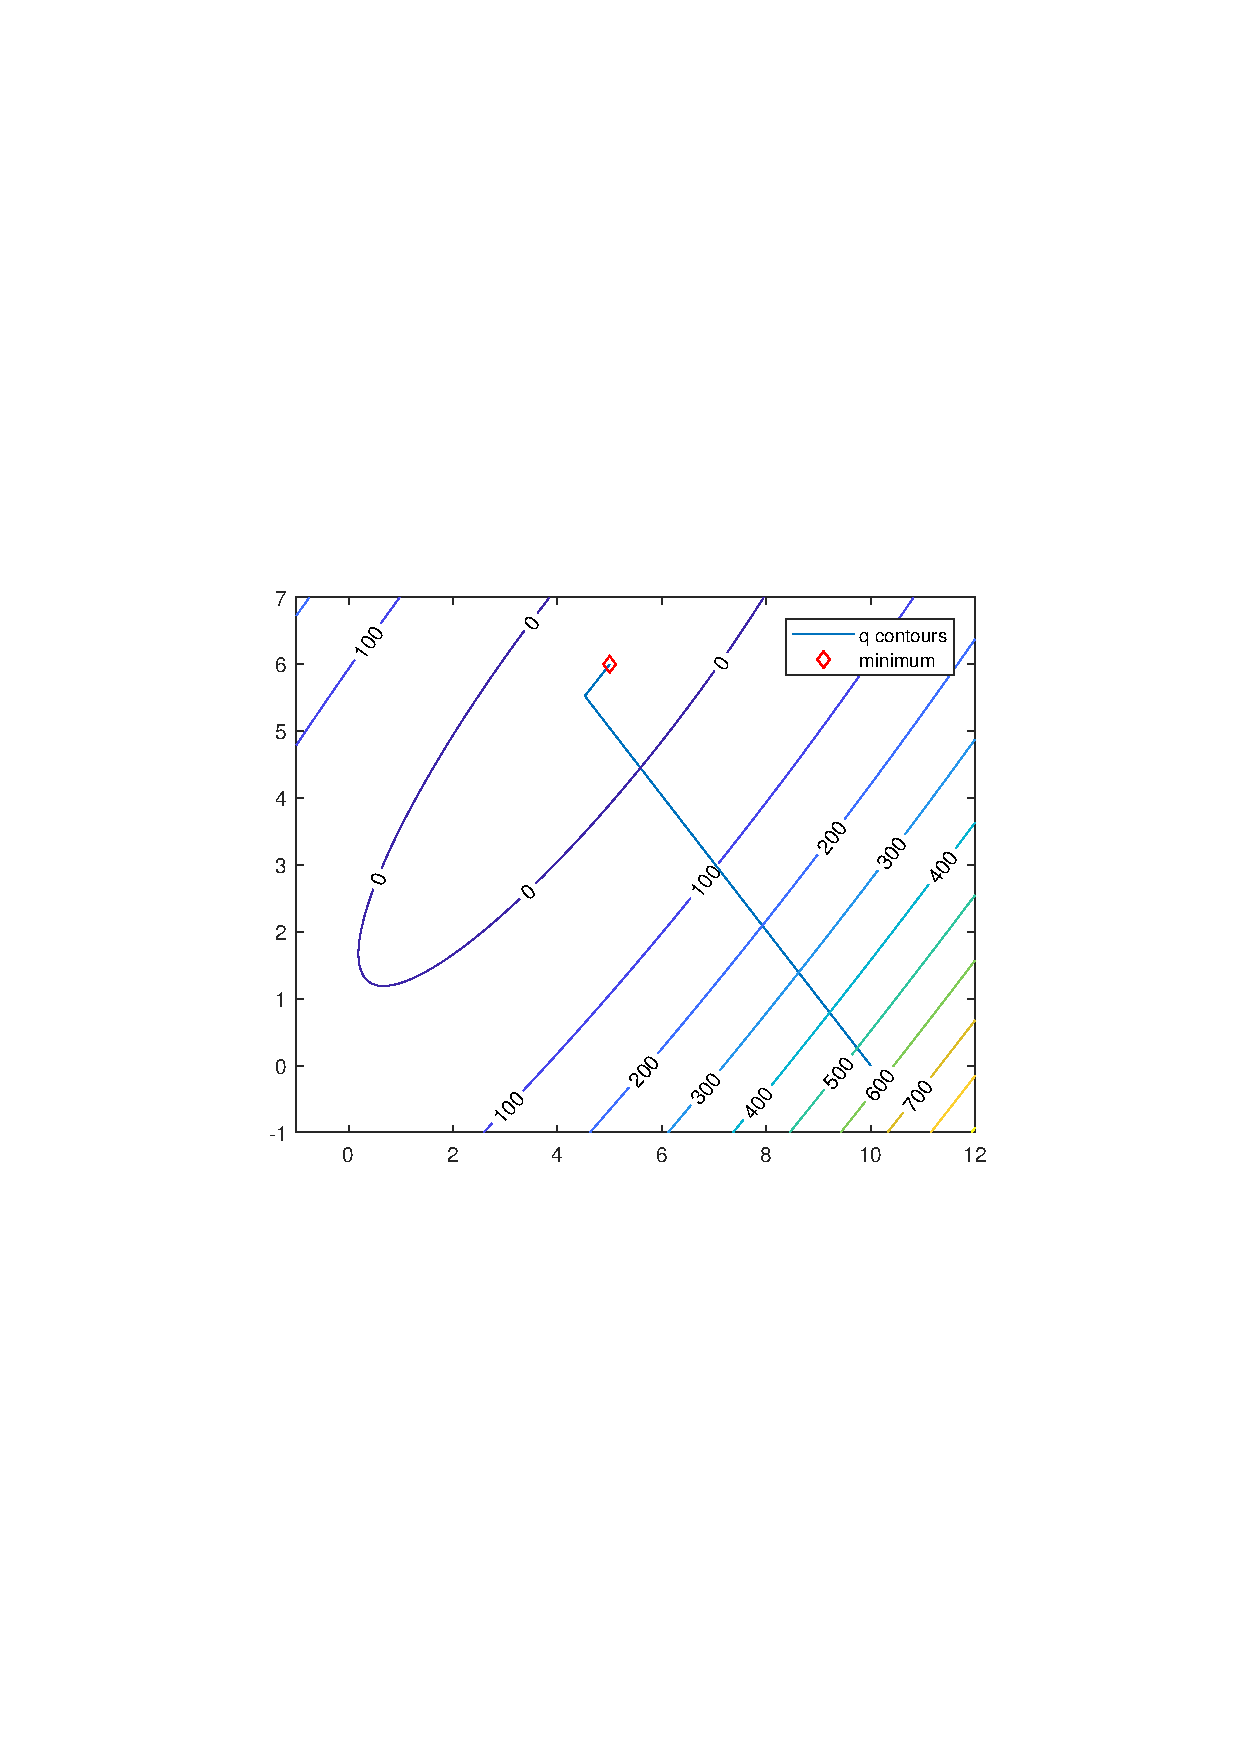
\includegraphics[width=5.7cm]{fig/1_3a.pdf}}
\subfigure{
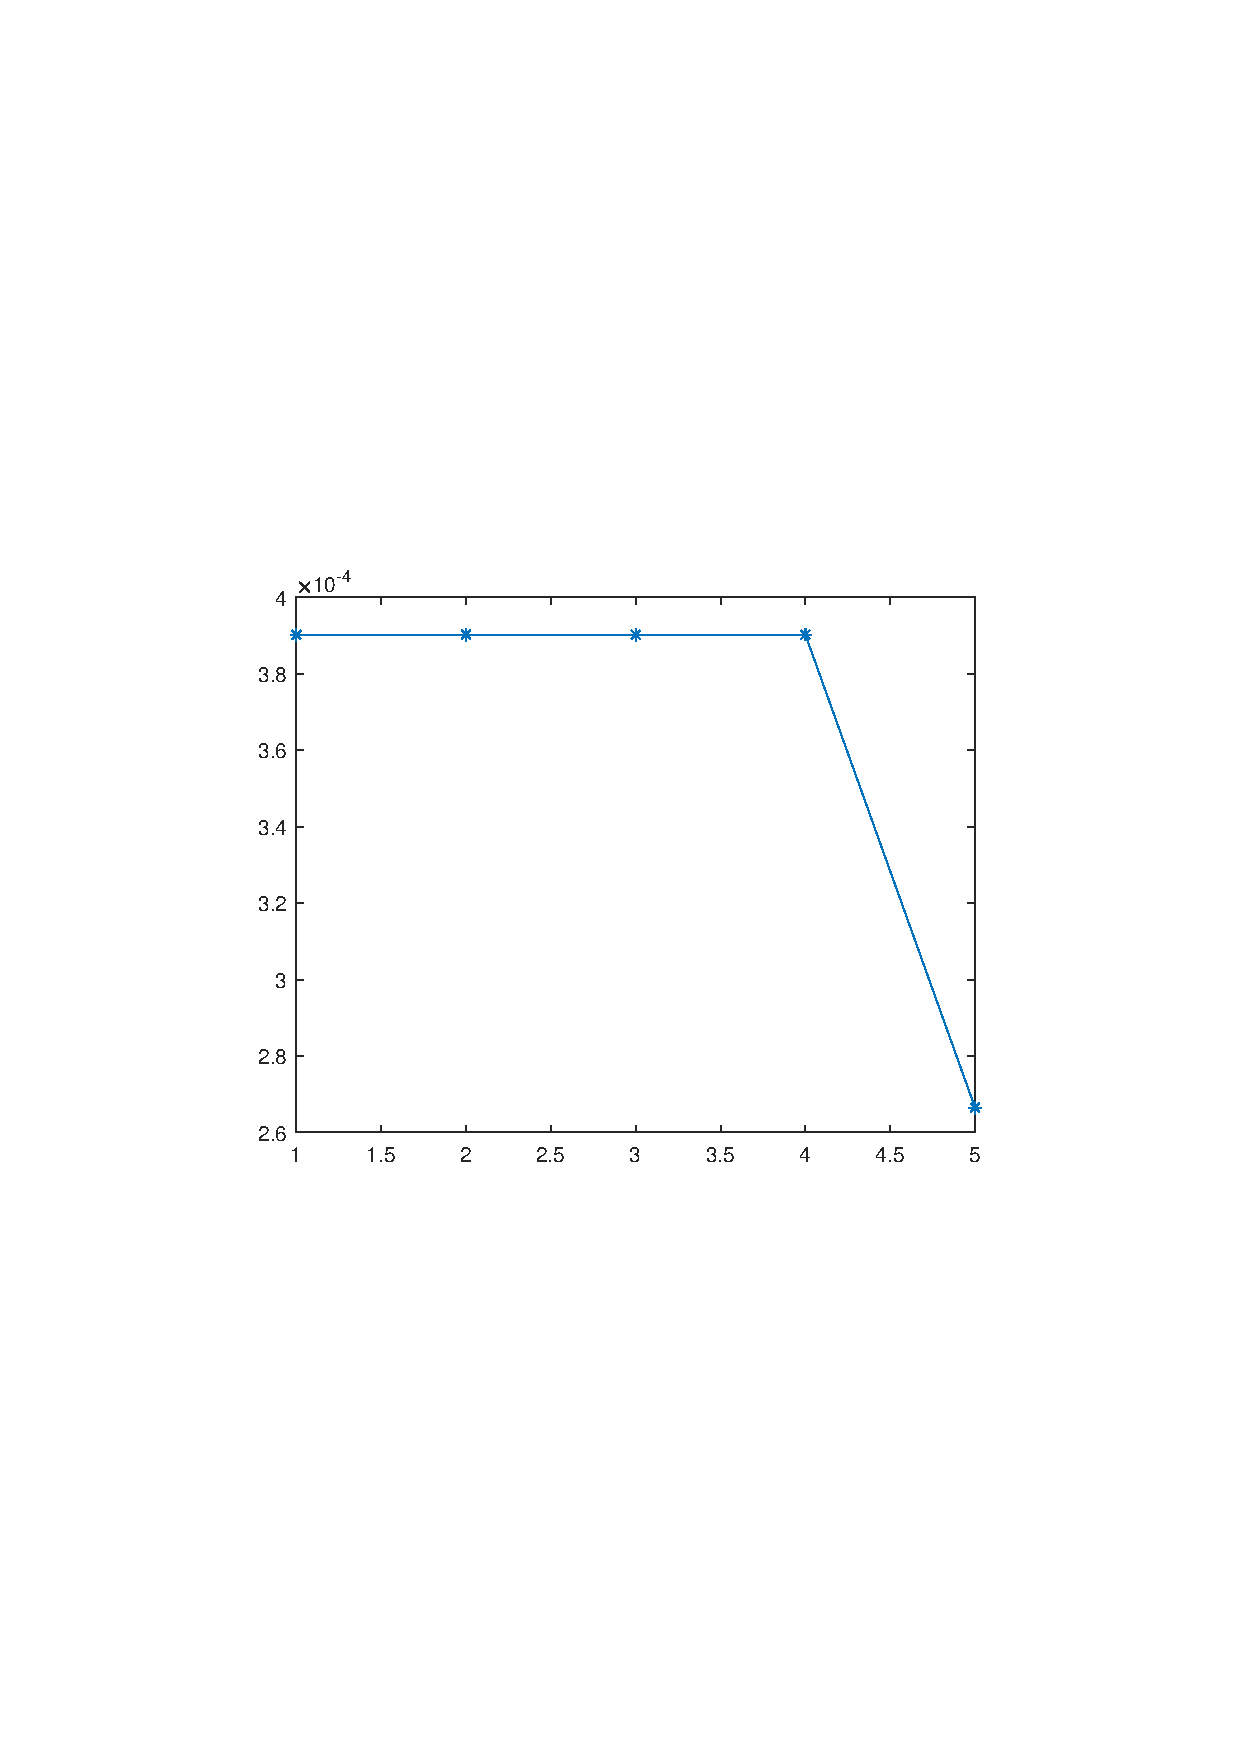
\includegraphics[width=5.8cm]{fig/1_3b.pdf}}
\caption{Steepest-denscent in (10,0)}
\label{Fig.lable}
\end{figure}

\begin{figure}[H]
\centering
\subfigure{
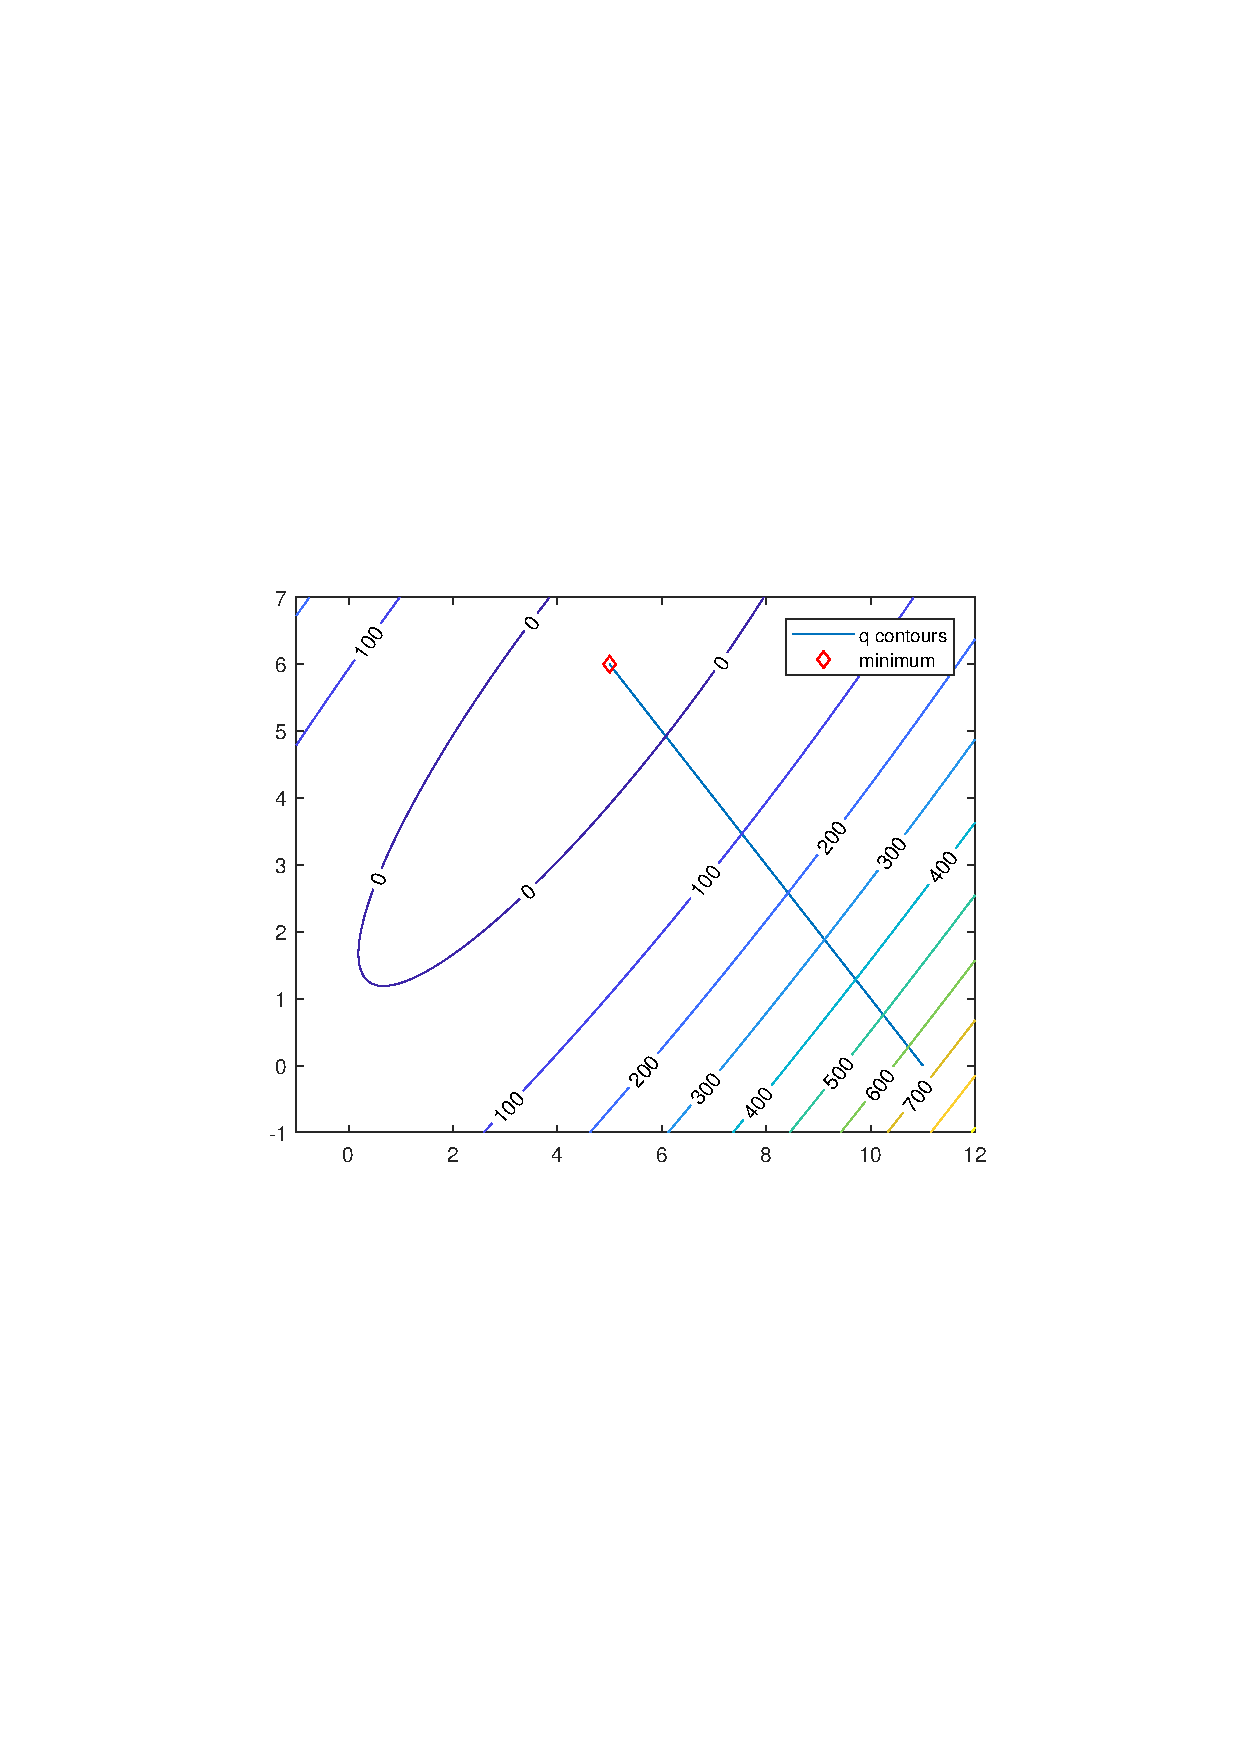
\includegraphics[width=5.8cm]{fig/1_4a.pdf}}
\subfigure{
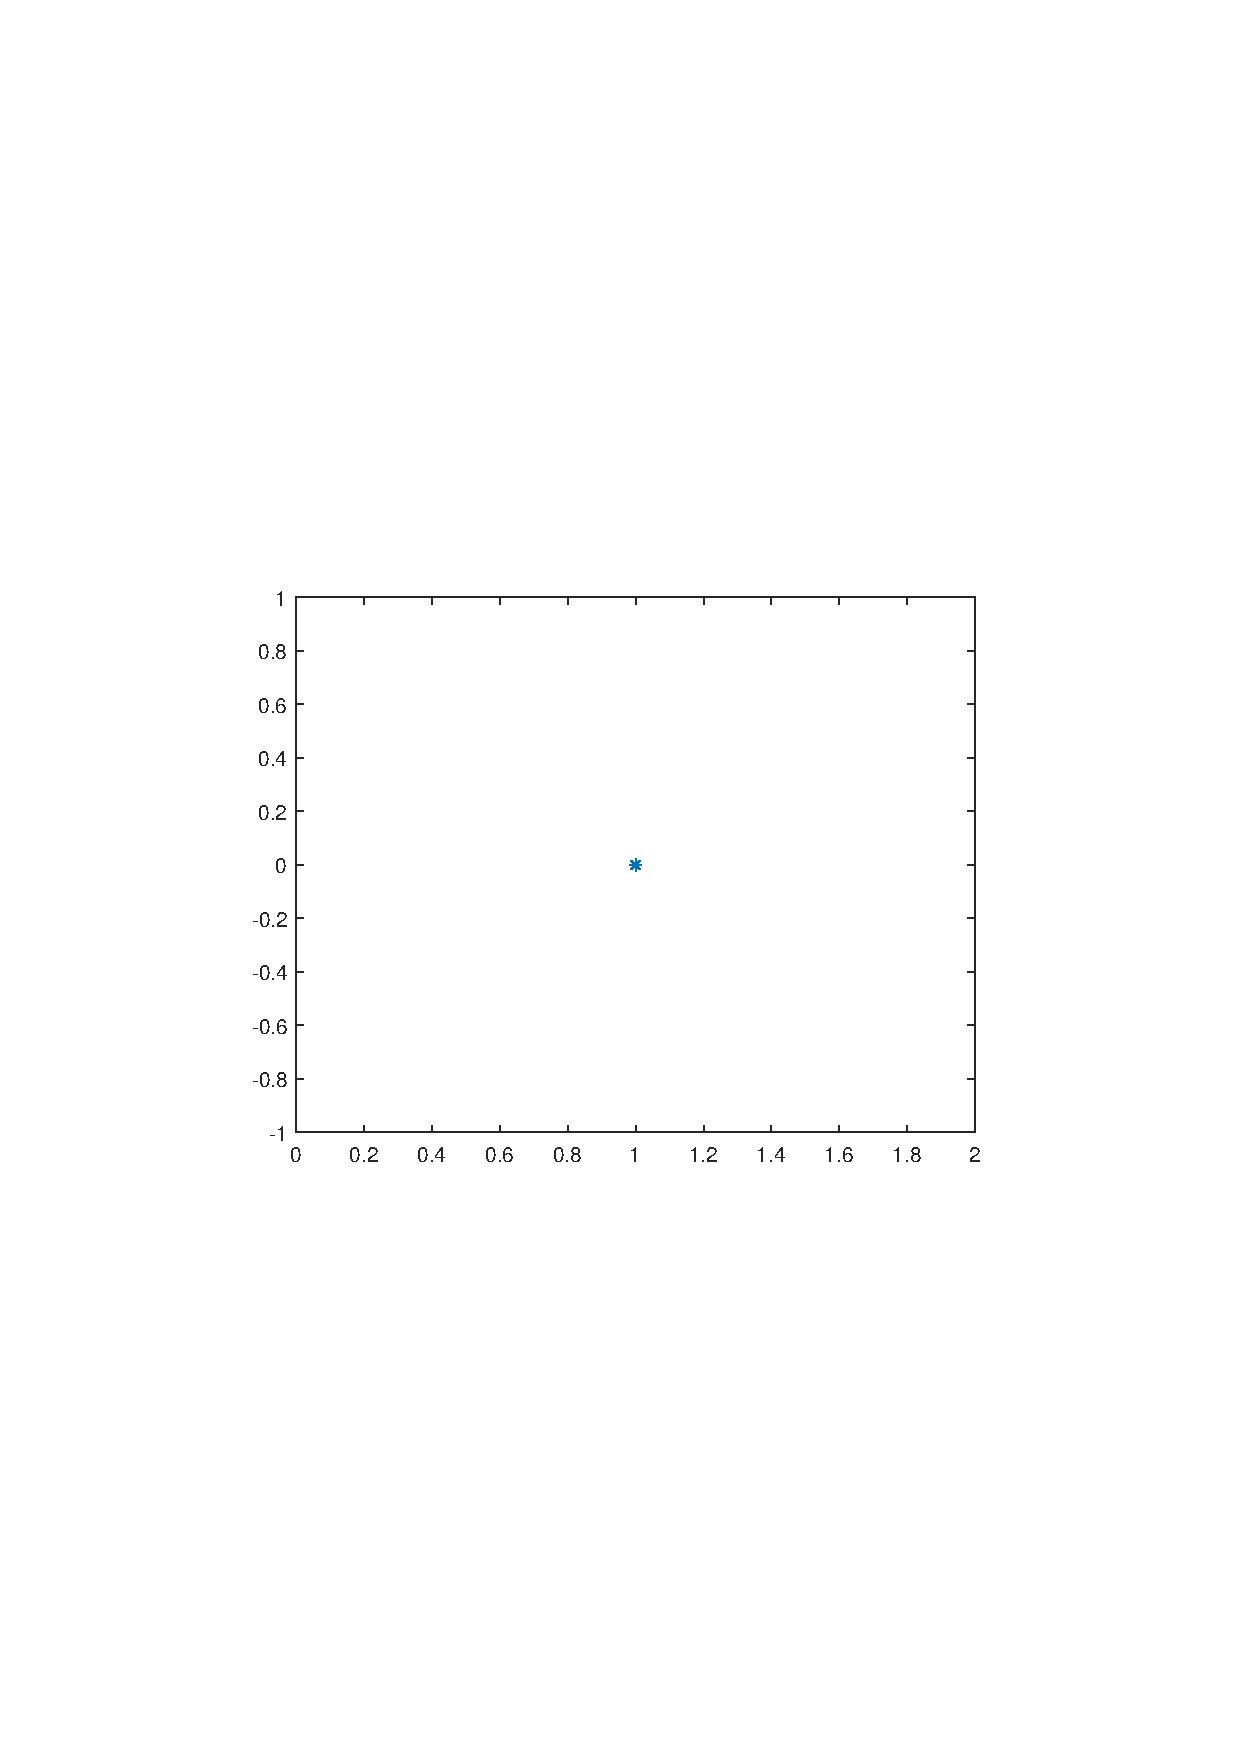
\includegraphics[width=5.9cm]{fig/1_4b.pdf}}

\caption{Steepest-denscent in (11,0)}
\label{Fig.lable}
\end{figure}

\begin{table}[H]
\centering
\caption{收敛因子比较}
	\begin{tabular}{ccccc}
	\toprule
	{起始点}&$(0,0)$&$(-0.4,0)$&$(10,0)$&$(11,0)$\\
	\midrule
	{收敛因子}&0.762255&0.810000&0.000390&0\\
	\bottomrule
	\end{tabular}
\end{table}

\newpage
\subsection{分析}
由于目标函数为凸函数,故使用梯度下降法从这四个不同的起始点出发都能收敛到全局最优点,然而线性收敛因子却互不相同.

由图像可知:在迭代开始后,函数值的收敛速度稳定在一个值左右,直到接近最优点时,收敛速度开始较大幅度波动。

而且,可以看出,初始点越接近等值线椭圆的狭长端,线性收敛因子越大,在点$(-0.4,0)$处甚至达到了线性收敛因子的上界0.81,而离狭长端越远,收敛因子越小。
这是由于梯度下降在构造搜索方向时没有充分利用到函数的二阶导数信息,在面临“峡谷”状的函数时,会反复震荡到“峡谷”的另一端,而不能直接向最优值方向前进。

容易看出,等值线椭圆的长轴端斜率为$9/10$,且$(-0.4,0)=(5,6)-0.6*(9,10)$,这说明点$(-0.4,0)$刚好处在等值线椭圆的长轴上,因此也是震荡最剧烈的地方,收敛速度达到了最坏收敛速度。